\documentclass[twoside,a4wide,12pt]{article}\usepackage[]{graphicx}\usepackage[]{color}
%% maxwidth is the original width if it is less than linewidth
%% otherwise use linewidth (to make sure the graphics do not exceed the margin)
\makeatletter
\def\maxwidth{ %
  \ifdim\Gin@nat@width>\linewidth
    \linewidth
  \else
    \Gin@nat@width
  \fi
}
\makeatother

\definecolor{fgcolor}{rgb}{0.345, 0.345, 0.345}
\newcommand{\hlnum}[1]{\textcolor[rgb]{0.686,0.059,0.569}{#1}}%
\newcommand{\hlstr}[1]{\textcolor[rgb]{0.192,0.494,0.8}{#1}}%
\newcommand{\hlcom}[1]{\textcolor[rgb]{0.678,0.584,0.686}{\textit{#1}}}%
\newcommand{\hlopt}[1]{\textcolor[rgb]{0,0,0}{#1}}%
\newcommand{\hlstd}[1]{\textcolor[rgb]{0.345,0.345,0.345}{#1}}%
\newcommand{\hlkwa}[1]{\textcolor[rgb]{0.161,0.373,0.58}{\textbf{#1}}}%
\newcommand{\hlkwb}[1]{\textcolor[rgb]{0.69,0.353,0.396}{#1}}%
\newcommand{\hlkwc}[1]{\textcolor[rgb]{0.333,0.667,0.333}{#1}}%
\newcommand{\hlkwd}[1]{\textcolor[rgb]{0.737,0.353,0.396}{\textbf{#1}}}%

\usepackage{framed}
\makeatletter
\newenvironment{kframe}{%
 \def\at@end@of@kframe{}%
 \ifinner\ifhmode%
  \def\at@end@of@kframe{\end{minipage}}%
  \begin{minipage}{\columnwidth}%
 \fi\fi%
 \def\FrameCommand##1{\hskip\@totalleftmargin \hskip-\fboxsep
 \colorbox{shadecolor}{##1}\hskip-\fboxsep
     % There is no \\@totalrightmargin, so:
     \hskip-\linewidth \hskip-\@totalleftmargin \hskip\columnwidth}%
 \MakeFramed {\advance\hsize-\width
   \@totalleftmargin\z@ \linewidth\hsize
   \@setminipage}}%
 {\par\unskip\endMakeFramed%
 \at@end@of@kframe}
\makeatother

\definecolor{shadecolor}{rgb}{.97, .97, .97}
\definecolor{messagecolor}{rgb}{0, 0, 0}
\definecolor{warningcolor}{rgb}{1, 0, 1}
\definecolor{errorcolor}{rgb}{1, 0, 0}
\newenvironment{knitrout}{}{} % an empty environment to be redefined in TeX

\usepackage{alltt}
%\DefineVerbatimEnvironment{Sinput}{Verbatim} {xleftmargin=2em,frame=single}
%\DefineVerbatimEnvironment{Soutput}{Verbatim} {xleftmargin=2em,frame=single}
\usepackage[left=2.5cm,top=2cm,right=2cm,bottom=2.5cm,bindingoffset=0.5cm]{geometry}
\usepackage{amsmath} 
\usepackage[affil-it]{authblk}
\usepackage{hyperref}
\usepackage{fullpage}
\usepackage{pdflscape}
\usepackage[backend=bibtex,sorting=none,style=ieee]{biblatex}
\usepackage{setspace}
\usepackage{inconsolata}
\bibliography{biblio}


\title{QSPR with 'camb'\\
{\bf C}hemically {\bf A}ware {\bf M}odel {\bf B}uilder\\
}

\author[1,3]{\rm Daniel Murrell\thanks{dsmurrell@gmail.com}}
\author[2,3]{\rm Isidro Cortes-Ciriano\thanks{isidrolauscher@gmail.com}} 
\affil[1]{Unilever Centre for Molecular Science Informatics, Department of Chemistry, University of Cambridge, Cambridge, United Kingdom.}
\affil[2]{Unite de Bioinformatique Structurale, Institut Pasteur and CNRS UMR 3825, Structural Biology and Chemistry Department, 25-28, rue Dr. Roux, 75 724 Paris, France.}
\affil[3]{Equal contributors}
\setlength{\parindent}{0pt}
\setlength{\parskip}{\baselineskip}%
\IfFileExists{upquote.sty}{\usepackage{upquote}}{}
\begin{document}

\maketitle
\onehalfspacing



\maketitle

In the following sections, we demonstrate the utility of the \texttt{camb} package by presenting a pipeline which generates various aqueous solubility models using 2D molecular descriptors calculated by the PaDEL-Descriptor package as input features. These models are then ensembled to create a single model with a greater predictive accuracy.

Firstly, the package needs to be loaded and the working directory set:

\begin{knitrout}
\definecolor{shadecolor}{rgb}{0.969, 0.969, 0.969}\color{fgcolor}\begin{kframe}
\begin{alltt}
\hlkwd{library}\hlstd{(camb)}
\hlkwd{setwd}\hlstd{(}\hlstr{'path_to_working_directory'}\hlstd{)}
\end{alltt}
\end{kframe}
\end{knitrout}

\section{Compounds}

\subsection{Reading and Preprocessing}
The compounds are read in and standardised. Internally, the Indigo C API \cite{Indigo}, which is incorporated into the \texttt{camb} package, is use to perform this task.
Molecules are represented with implicit hydrogens, dearomatized, and passed through the InChI format to ensure that tautomers are represented by the same SMILES.

The \texttt{StandardiseMolecules} function enables the representation of molecular structures in a similarly processed form.
The different arguments of this function allow control over the maximum number of (i) fluorines, (ii) chlorines,
(iii) bromines, and (iv) iodines the molecule contains in order to be retained for training.
Inorgnaic molecules (those containing atoms not in \{H, C, N, O, P, S, F, Cl, Br, I\}) are removed if the argument \texttt{remove.inorganic} is set to \texttt{TRUE}. This is the function's default behaviour.
The upper and lower limits for the molecular mass can be set with the arguments \texttt{min.mass.limit} and \texttt{max.mass.limit}.
The name of the file containing the chemical structures is input to the argument \texttt{structures.file}.
\begin{knitrout}
\definecolor{shadecolor}{rgb}{0.969, 0.969, 0.969}\color{fgcolor}\begin{kframe}
\begin{alltt}
\hlkwd{StandardiseMolecules}\hlstd{(}\hlkwc{structures.file}\hlstd{=}\hlstr{"solubility_2007_ref2.sdf"}\hlstd{,}
                     \hlkwc{standardised.file}\hlstd{=}\hlstr{"standardised.sdf"}\hlstd{,}
                     \hlkwc{removed.file}\hlstd{=}\hlstr{"removed.sdf"}\hlstd{,}
                     \hlkwc{properties.file} \hlstd{=} \hlstr{"properties.csv"}\hlstd{,}
                     \hlkwc{remove.inorganic}\hlstd{=}\hlnum{TRUE}\hlstd{,}
                     \hlkwc{fluorine.limit}\hlstd{=}\hlnum{3}\hlstd{,}
                     \hlkwc{chlorine.limit}\hlstd{=}\hlnum{3}\hlstd{,}
                     \hlkwc{bromine.limit}\hlstd{=}\hlnum{3}\hlstd{,}
                     \hlkwc{iodine.limit}\hlstd{=}\hlnum{3}\hlstd{,}
                     \hlkwc{min.mass.limit}\hlstd{=}\hlnum{20}\hlstd{,}
                     \hlkwc{max.mass.limit}\hlstd{=}\hlnum{900}\hlstd{)}
\end{alltt}
\end{kframe}
\end{knitrout}
Molecules that Indigo manages to parse and that pass the filters are written to the file indicated in the argument "standardised.file". Molecules that are discarded for training purposes are written to the file indicated in the "removed.file" argument.

\section{Target Visualisation}
The properties specified in the structure file of all molecules and an index, in the column "kept", indicating which molecules were deleted (0) and kept (1),
are written to the file indicated in the argument "properties.file" which is in CSV format.
In this case the file is \verb|"properties.csv"|.
\begin{knitrout}
\definecolor{shadecolor}{rgb}{0.969, 0.969, 0.969}\color{fgcolor}\begin{kframe}
\begin{alltt}
\hlstd{properties} \hlkwb{<-} \hlkwd{read.table}\hlstd{(}\hlstr{"properties.csv"}\hlstd{,} \hlkwc{header}\hlstd{=}\hlnum{TRUE}\hlstd{,} \hlkwc{sep}\hlstd{=}\hlstr{"\textbackslash{}t"}\hlstd{)}
\hlstd{properties} \hlkwb{<-} \hlstd{properties[properties}\hlopt{$}\hlstd{Kept}\hlopt{==}\hlnum{1}\hlstd{, ]}
\hlkwd{head}\hlstd{(properties)}
\hlstd{targets} \hlkwb{<-} \hlkwd{data.frame}\hlstd{(}\hlkwc{Name} \hlstd{= properties}\hlopt{$}\hlstd{NAME,} \hlkwc{target} \hlstd{= properties}\hlopt{$}\hlstd{EXPT)}
\hlstd{p} \hlkwb{<-} \hlkwd{DensityResponse}\hlstd{(targets}\hlopt{$}\hlstd{target)} \hlopt{+} \hlkwd{xlab}\hlstd{(}\hlstr{"LogS Target Distribution"}\hlstd{)}
\hlstd{p}
\end{alltt}
\end{kframe}\begin{figure}[]


{\centering 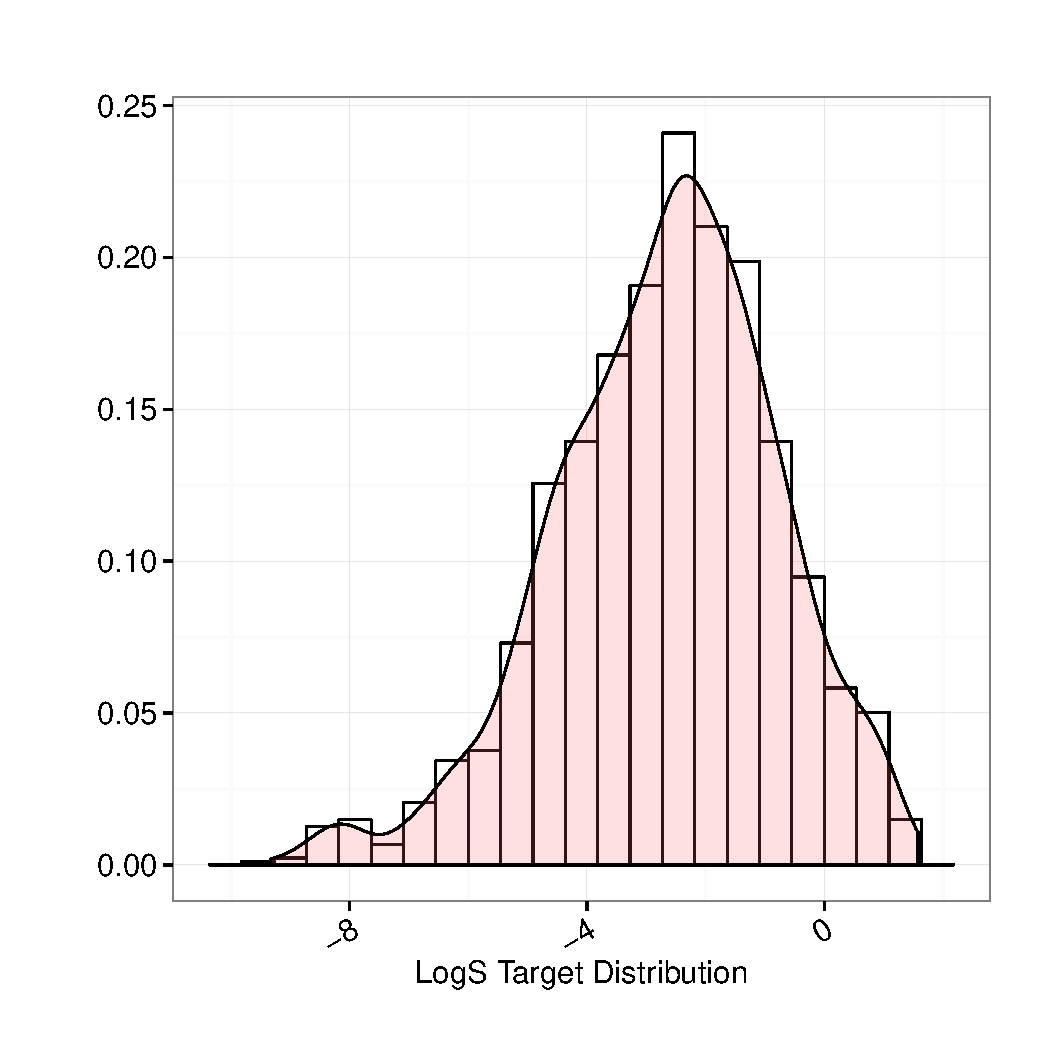
\includegraphics[width=8cm]{figure/unnamed-chunk-5} 

}

\caption[LogS Target Distribution]{LogS Target Distribution\label{fig:unnamed-chunk-5}}
\end{figure}


\end{knitrout}

\subsection{PaDEL Descriptors}
One and two-dimensional PaDEL\cite{padel} descriptors and fingerprints can be calculated with the function "GeneratePadelDescriptors":
\begin{knitrout}
\definecolor{shadecolor}{rgb}{0.969, 0.969, 0.969}\color{fgcolor}\begin{kframe}
\begin{alltt}
\hlstd{descriptors} \hlkwb{<-} \hlkwd{GeneratePadelDescriptors}\hlstd{(}\hlkwc{standardised.file} \hlstd{=} \hlstr{"standardised.sdf"}\hlstd{,}
    \hlkwc{types} \hlstd{=} \hlkwd{c}\hlstd{(}\hlstr{"2D"}\hlstd{),} \hlkwc{threads} \hlstd{=} \hlnum{1}\hlstd{)}
\hlstd{descriptors} \hlkwb{<-} \hlkwd{RemoveStandardisedPrefix}\hlstd{(descriptors)}
\hlkwd{saveRDS}\hlstd{(descriptors,} \hlkwc{file} \hlstd{=} \hlstr{"descriptors.rds"}\hlstd{)}
\end{alltt}
\end{kframe}
\end{knitrout}


\section{Statistical Pre-processing}
Merge the calculated descriptors and the target values by name into a single data.frame. Check that the number of rows of the merged and original data.frames are the same. Split the data.frame into \textit{ids}, \textit{x} and \textit{y} where \textit{ids} are the molecule names, \textit{x} are the descriptor values and \textit{y} is the target values.  
\begin{knitrout}
\definecolor{shadecolor}{rgb}{0.969, 0.969, 0.969}\color{fgcolor}\begin{kframe}
\begin{alltt}
\hlstd{all} \hlkwb{<-} \hlkwd{merge}\hlstd{(}\hlkwc{x} \hlstd{= targets,} \hlkwc{y} \hlstd{= descriptors,} \hlkwc{by} \hlstd{=} \hlstr{"Name"}\hlstd{)}
\hlstd{ids} \hlkwb{<-} \hlstd{all}\hlopt{$}\hlstd{Name}
\hlstd{x} \hlkwb{<-} \hlstd{all[}\hlnum{3}\hlopt{:}\hlkwd{ncol}\hlstd{(all)]}
\hlstd{y} \hlkwb{<-} \hlstd{all}\hlopt{$}\hlstd{target}
\end{alltt}
\end{kframe}
\end{knitrout}

Sometimes, some descriptors are not calculated for all molecules, thus giving a "NA" or "Inf" as descriptor value.
Instead of removing that descriptor for all molecules, the missing descriptor values can be imputed from the corresponding descriptor values of the rest of molecules.
Descriptor values equal to "Inf" are converted to "NA".
For the imputation of missing descriptor values, the R package {\it impute} is required.
Depending on the R version, it can be accessed from either {\it CRAN} or {\it Bioconductor}.
\begin{knitrout}
\definecolor{shadecolor}{rgb}{0.969, 0.969, 0.969}\color{fgcolor}\begin{kframe}
\begin{alltt}
\hlstd{x.finite} \hlkwb{<-} \hlkwd{ReplaceInfinitesWithNA}\hlstd{(x)}
\hlstd{x.imputed} \hlkwb{<-} \hlkwd{ImputeFeatures}\hlstd{(x.finite)}
\end{alltt}


{\ttfamily\noindent\itshape\color{messagecolor}{\#\# Loading required package: impute}}\begin{verbatim}
## Cluster size 1606 broken into 375 1231 
## Done cluster 375 
## Done cluster 1231
\end{verbatim}
\end{kframe}
\end{knitrout}

Split the dataset into a training (80\%) and a holdout (20\%) set that will be used to assess the predictive ability of the models. Remove the following descriptors: (i) those with a variance close to zero (near-zero variance), and (ii) those highly correlated:
\begin{knitrout}
\definecolor{shadecolor}{rgb}{0.969, 0.969, 0.969}\color{fgcolor}\begin{kframe}
\begin{alltt}
\hlstd{dataset} \hlkwb{<-} \hlkwd{SplitSet}\hlstd{(ids, x.imputed, y,} \hlkwc{percentage} \hlstd{=} \hlnum{20}\hlstd{)}
\hlstd{dataset} \hlkwb{<-} \hlkwd{RemoveNearZeroVarianceFeatures}\hlstd{(dataset,}
    \hlkwc{frequencyCutoff} \hlstd{=} \hlnum{30}\hlstd{)}
\end{alltt}


{\ttfamily\noindent\itshape\color{messagecolor}{\#\# 397 features removed with variance below cutoff}}\begin{alltt}
\hlstd{dataset} \hlkwb{<-} \hlkwd{RemoveHighlyCorrelatedFeatures}\hlstd{(dataset,}
    \hlkwc{correlationCutoff} \hlstd{=} \hlnum{0.95}\hlstd{)}
\end{alltt}


{\ttfamily\noindent\itshape\color{messagecolor}{\#\# 121 features removed with correlation above cutoff}}\end{kframe}
\end{knitrout}

Convert the descriptors to z-scores by centering them to have a mean of zero and scaling them to have unit variance:
\begin{knitrout}
\definecolor{shadecolor}{rgb}{0.969, 0.969, 0.969}\color{fgcolor}\begin{kframe}
\begin{alltt}
\hlstd{dataset} \hlkwb{<-} \hlkwd{PreProcess}\hlstd{(dataset)}
\end{alltt}
\end{kframe}
\end{knitrout}

Given that cross-validation (CV) will be used to optimize the hyperparameters of the models, we divide the training set in 5 folds:
\begin{knitrout}
\definecolor{shadecolor}{rgb}{0.969, 0.969, 0.969}\color{fgcolor}\begin{kframe}
\begin{alltt}
\hlstd{dataset} \hlkwb{<-} \hlkwd{GetCVTrainControl}\hlstd{(dataset)}
\hlkwd{saveRDS}\hlstd{(dataset,} \hlkwc{file} \hlstd{=} \hlstr{"dataset_logS_preprocessed.rds"}\hlstd{)}
\end{alltt}
\end{kframe}
\end{knitrout}

All models are trained with the same CV options, {\it i.e.} the arguments of the function 'GetCVTrainControl' to allow ensemble modeling (see below).
It is important to mention that the functions presented in the previous code blocks depend on functions from the {\it caret} package, namely: 
\begin{itemize}
\item RemoveNearZeroVarianceFeatures : nearZeroVar
\item RemoveHighlyCorrelatedFeatures : findCorrelation
\item PreProcess : preProcess
\item GetCVTrainControl : trainControl
\end{itemize}
Experienced users might want to control more arguments of the underlying {\it caret} functions.
This is certainly possible as the arguments given to the {\it camb} functions will be subsequently given to the {\it caret} counterparts.
The default values of these function however permit the less experienced user to fo throught the statistical preprocessing
steps with ease, though guaranteeing that the choice of the argument values is reasonable.

\section{Model Training}

In the following section we will present the different steps required to train a QSPR model with {\it camb}. It should be noted that the above steps can be run locally on a low powered computer such as a laptop and the preprocessed dataset saved to disk. This can then be copied to a high powered machine with multiple cores for model training and the resulting models saved back to the local machine. Pro tip: Dropbox can be used to sync this proceedure so that manual transfer is not required.

\begin{knitrout}
\definecolor{shadecolor}{rgb}{0.969, 0.969, 0.969}\color{fgcolor}\begin{kframe}
\begin{alltt}
\hlstd{dataset} \hlkwb{<-} \hlkwd{readRDS}\hlstd{(}\hlstr{"dataset_logS_preprocessed.rds"}\hlstd{)}
\hlcom{# register the number of cores to use in training}
\hlkwd{registerDoMC}\hlstd{(}\hlkwc{cores} \hlstd{=} \hlnum{10}\hlstd{)}
\end{alltt}
\end{kframe}
\end{knitrout}

\subsection{Support Vector Machines (SVM)}
Firstly, a SVM will be trained\cite{svmreview}.
We define an exponential grid (base 2) to optimize the hyperparameters. The \texttt{train} function from the \texttt{caret} package is used directly for model training.

\begin{knitrout}
\definecolor{shadecolor}{rgb}{0.969, 0.969, 0.969}\color{fgcolor}\begin{kframe}
\begin{alltt}
\hlstd{method} \hlkwb{<-} \hlstr{"svmRadial"}
\hlstd{tune.grid} \hlkwb{<-} \hlkwd{expand.grid}\hlstd{(}\hlkwc{.sigma} \hlstd{=} \hlkwd{expGrid}\hlstd{(}\hlopt{-}\hlnum{8}\hlstd{,} \hlnum{4}\hlstd{,} \hlnum{2}\hlstd{,}
    \hlnum{2}\hlstd{),} \hlkwc{.C} \hlstd{=} \hlkwd{c}\hlstd{(}\hlnum{1e-04}\hlstd{,} \hlnum{0.001}\hlstd{,} \hlnum{0.01}\hlstd{,} \hlnum{0.1}\hlstd{,} \hlnum{1}\hlstd{,} \hlnum{10}\hlstd{,} \hlnum{100}\hlstd{))}
\hlstd{model} \hlkwb{<-} \hlkwd{train}\hlstd{(dataset}\hlopt{$}\hlstd{x.train, dataset}\hlopt{$}\hlstd{y.train, method,}
    \hlkwc{tuneGrid} \hlstd{= tune.grid,} \hlkwc{trControl} \hlstd{= dataset}\hlopt{$}\hlstd{trControl)}
\hlkwd{saveRDS}\hlstd{(model,} \hlkwc{file} \hlstd{=} \hlkwd{paste}\hlstd{(method,} \hlstr{".rds"}\hlstd{,} \hlkwc{sep} \hlstd{=} \hlstr{""}\hlstd{))}
\end{alltt}
\end{kframe}
\end{knitrout}

\subsection{Random Forest}
We proceed similarly in the case of a random forest (RF) model\cite{rf}.

\begin{knitrout}
\definecolor{shadecolor}{rgb}{0.969, 0.969, 0.969}\color{fgcolor}\begin{kframe}
\begin{alltt}
\hlstd{method} \hlkwb{<-} \hlstr{"rf"}
\hlstd{tune.grid} \hlkwb{<-} \hlkwd{expand.grid}\hlstd{(}\hlkwc{.mtry} \hlstd{=} \hlkwd{seq}\hlstd{(}\hlnum{5}\hlstd{,} \hlnum{100}\hlstd{,} \hlnum{5}\hlstd{))}
\hlstd{model} \hlkwb{<-} \hlkwd{train}\hlstd{(dataset}\hlopt{$}\hlstd{x.train, dataset}\hlopt{$}\hlstd{y.train, method,}
    \hlkwc{tuneGrid} \hlstd{= tune.grid,} \hlkwc{trControl} \hlstd{= dataset}\hlopt{$}\hlstd{trControl)}
\hlkwd{saveRDS}\hlstd{(model,} \hlkwc{file} \hlstd{=} \hlkwd{paste}\hlstd{(method,} \hlstr{".rds"}\hlstd{,} \hlkwc{sep} \hlstd{=} \hlstr{""}\hlstd{))}
\end{alltt}
\end{kframe}
\end{knitrout}

\subsection{Gradient Boosting Machine}
We proceed similarly in the case of a gradient boosting machine (GBM) model\cite{gbm}.

\begin{knitrout}
\definecolor{shadecolor}{rgb}{0.969, 0.969, 0.969}\color{fgcolor}\begin{kframe}
\begin{alltt}
\hlstd{method} \hlkwb{<-} \hlstr{"gbm"}
\hlstd{tune.grid} \hlkwb{<-} \hlkwd{expand.grid}\hlstd{(}\hlkwc{.n.trees} \hlstd{=} \hlkwd{c}\hlstd{(}\hlnum{500}\hlstd{,} \hlnum{1000}\hlstd{),} \hlkwc{.interaction.depth} \hlstd{=} \hlkwd{c}\hlstd{(}\hlnum{25}\hlstd{),}
    \hlkwc{.shrinkage} \hlstd{=} \hlkwd{c}\hlstd{(}\hlnum{0.01}\hlstd{,} \hlnum{0.02}\hlstd{,} \hlnum{0.04}\hlstd{,} \hlnum{0.08}\hlstd{))}
\hlstd{model} \hlkwb{<-} \hlkwd{train}\hlstd{(dataset}\hlopt{$}\hlstd{x.train, dataset}\hlopt{$}\hlstd{y.train, method,}
    \hlkwc{tuneGrid} \hlstd{= tune.grid,} \hlkwc{trControl} \hlstd{= dataset}\hlopt{$}\hlstd{trControl)}
\hlkwd{saveRDS}\hlstd{(model,} \hlkwc{file} \hlstd{=} \hlkwd{paste}\hlstd{(method,} \hlstr{".rds"}\hlstd{,} \hlkwc{sep} \hlstd{=} \hlstr{""}\hlstd{))}
\end{alltt}
\end{kframe}
\end{knitrout}

Determine if your hyper-parameter search needs to be altered. In the following we focus on the RF model, though the same steps can be applied to the GBM and SVM models. If your hyper-parameters lead you to what looks like a global minimum then you can stop scanning the space of hyper-parameters, otherwise you need to adjust the grid and retrain your model.
\begin{knitrout}
\definecolor{shadecolor}{rgb}{0.969, 0.969, 0.969}\color{fgcolor}\begin{kframe}
\begin{alltt}
\hlstd{model} \hlkwb{<-} \hlkwd{readRDS}\hlstd{(}\hlstr{"rf.rds"}\hlstd{)}
\hlkwd{plot}\hlstd{(model,} \hlkwc{metric} \hlstd{=} \hlstr{"RMSE"}\hlstd{)}
\end{alltt}
\end{kframe}\begin{figure}[]


{\centering 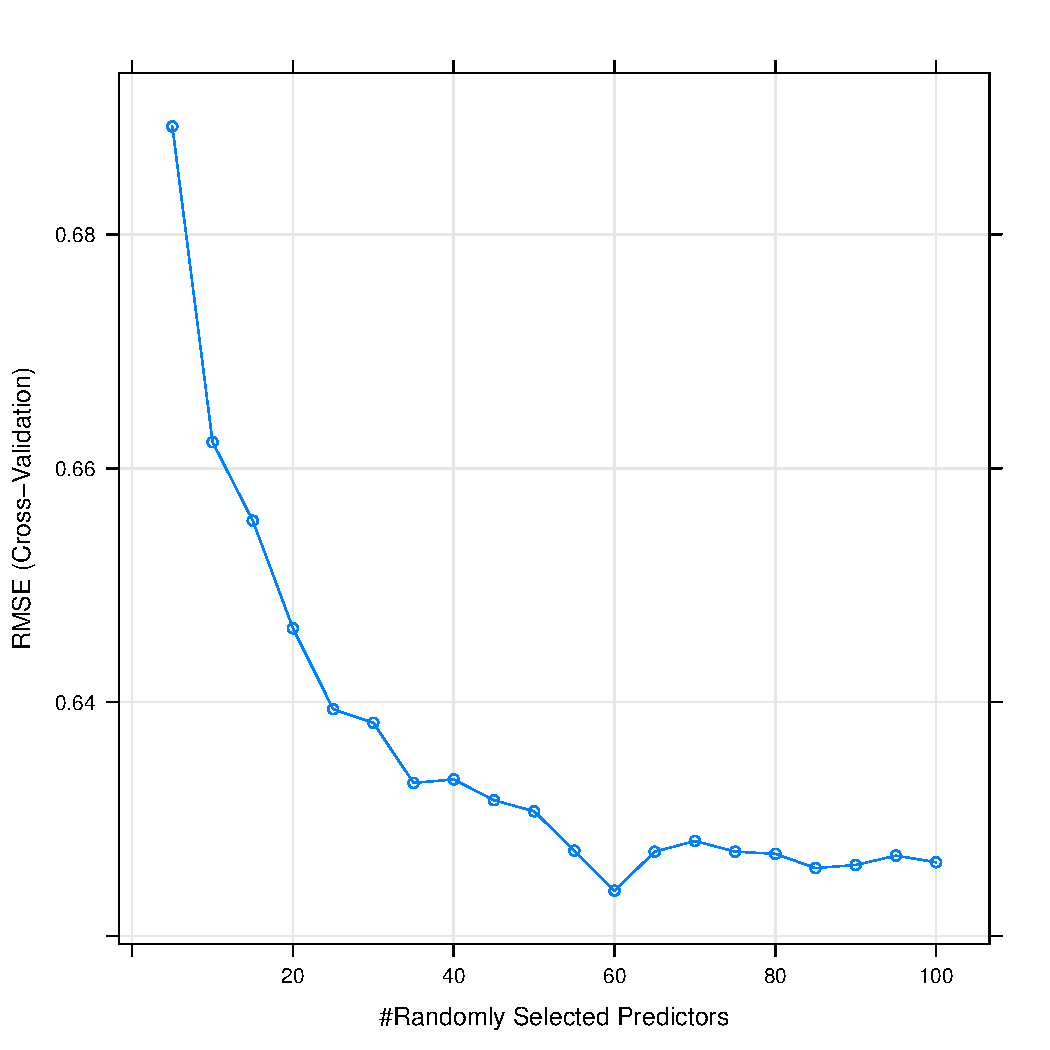
\includegraphics[width=8cm]{figure/unnamed-chunk-17} 

}

\caption[CV RMSE over the hyperparameters]{CV RMSE over the hyperparameters\label{fig:unnamed-chunk-17}}
\end{figure}


\end{knitrout}

\section{Model Evaluation}

Once the models are trained, the cross validated metrics can be calculated:
We assume that the metric used for the choice of the best combination of hyperparameters is 'RMSE',
which is normally considered as the aim of bioactivity modeling, {\it i.e.} how far (on average) are our 
predictions from the real the bioactivity values?.

\begin{knitrout}
\definecolor{shadecolor}{rgb}{0.969, 0.969, 0.969}\color{fgcolor}\begin{kframe}
\begin{alltt}
\hlkwd{print}\hlstd{(}\hlkwd{RMSE_CV}\hlstd{(model,} \hlkwc{digits} \hlstd{=} \hlnum{3}\hlstd{))}
\end{alltt}


{\ttfamily\noindent\bfseries\color{errorcolor}{\#\# Error: could not find function "{}RMSE\_CV"{}}}\begin{alltt}
\hlkwd{print}\hlstd{(}\hlkwd{Rsquared_CV}\hlstd{(model,} \hlkwc{digits} \hlstd{=} \hlnum{3}\hlstd{))}
\end{alltt}


{\ttfamily\noindent\bfseries\color{errorcolor}{\#\# Error: could not find function "{}Rsquared\_CV"{}}}\end{kframe}
\end{knitrout}

\section{Bibliography}
\printbibliography

\end{document}
